\documentclass[12pt]{report}
\usepackage[utf8]{inputenc}
\usepackage[english, russian]{babel}
\usepackage{listings}
\usepackage{graphicx}
\usepackage{float}
\graphicspath{{imgs/}}
\usepackage{amsmath,amsfonts,amssymb,amsthm,mathtools} 
\usepackage{pgfplots}
\usepackage{filecontents}
\usepackage{indentfirst}
\usepackage{eucal}
\usepackage{enumitem}
\frenchspacing

\usepackage{indentfirst} % Красная строка

\usetikzlibrary{datavisualization}
\usetikzlibrary{datavisualization.formats.functions}

\usepackage{amsmath}
\usepackage{fixltx2e}


\definecolor{bluekeywords}{rgb}{0,0,1}
\definecolor{greencomments}{rgb}{0,0.5,0}
\definecolor{redstrings}{rgb}{0.64,0.08,0.08}
\definecolor{xmlcomments}{rgb}{0.5,0.5,0.5}
\definecolor{types}{rgb}{0.17,0.57,0.68}

\usepackage{listings}
\lstset{language=[Sharp]C,
	captionpos=t,
	numbers=left, %Nummerierung
	numberstyle=\small, % kleine Zeilennummern
	frame=single, % Oberhalb und unterhalb des Listings ist eine Linie
	stepnumber=1,                   
	numbersep=5pt,                
	showspaces=false,
	tabsize=2,
	showtabs=false,
	breaklines=true,
	showstringspaces=false,
	breakatwhitespace=true,
	escapeinside={(*@}{@*)},
	commentstyle=\color{greencomments},
	morekeywords={partial, var, value, get, set},
	keywordstyle=\color{bluekeywords},
	stringstyle=\color{redstrings},
	basicstyle=\ttfamily\small,
}

\usepackage[left=2cm,right=2cm, top=2cm,bottom=2cm,bindingoffset=0cm]{geometry}
% Для измененных титулов глав:
\usepackage{titlesec, blindtext, color} % подключаем нужные пакеты
\definecolor{gray75}{gray}{0.75} % определяем цвет
\newcommand{\hsp}{\hspace{20pt}} % длина линии в 20pt
% titleformat определяет стиль
\titleformat{\chapter}[hang]{\Huge\bfseries}{\thechapter\hsp\textcolor{gray75}{|}\hsp}{0pt}{\Huge\bfseries}


% plot
\usepackage{pgfplots}
\usepackage{filecontents}
\usetikzlibrary{datavisualization}
\usetikzlibrary{datavisualization.formats.functions}
 
\begin{document}
  %\def\chaptername{} % убирает "Глава"
\thispagestyle{empty}
\begin{titlepage}
	\noindent \begin{minipage}{0.15\textwidth}
	
\includegraphics[width=\linewidth]{b_logo}
	\end{minipage}
	\noindent\begin{minipage}{0.9\textwidth}\centering
		\textbf{Министерство науки и высшего образования Российской Федерации}\\
		\textbf{Федеральное государственное бюджетное образовательное учреждение высшего образования}\\
		\textbf{~~~«Московский государственный технический университет имени Н.Э.~Баумана}\\
		\textbf{(национальный исследовательский университет)»}\\
		\textbf{(МГТУ им. Н.Э.~Баумана)}
	\end{minipage}
	
	\noindent\rule{18cm}{3pt}
	\newline\newline
	\noindent ФАКУЛЬТЕТ $\underline{\text{«Информатика и системы управления»}}$ \newline\newline
	\noindent КАФЕДРА $\underline{\text{«Программное обеспечение ЭВМ и информационные технологии»}}$\newline\newline\newline\newline\newline\newline\newline\newline\newline\newline\newline
	
	
	\begin{center}
		\noindent\begin{minipage}{1.3\textwidth}\centering
			\Large\textbf{  Домашнее задание }\newline
			\textbf{по дисциплине "Анализ алгоритмов"}\newline\newline
		\end{minipage}
	\end{center}
	
	\noindent\textbf{Тема} $\underline{\text{Графовые модели программ}}$\newline\newline
	\noindent\textbf{Студент} $\underline{\text{Малышев И. А.}}$\newline\newline
	\noindent\textbf{Группа} $\underline{\text{ИУ7-51Б}}$\newline\newline
	\noindent\textbf{Оценка (баллы)} $\underline{\text{~~~~~~~~~~~~~~~~~~~~~~~~~~~}}$\newline\newline
	\noindent\textbf{Преподаватель: } $\underline{\text{Волкова Л. Л.}}$\newline\newline\newline
	
	\begin{center}
		\vfill
		Москва~---~\the\year
		~г.
	\end{center}
\end{titlepage}


\tableofcontents
  
\chapter{Исходный код алгоритма}

\begin{lstlisting}[label=some-code,caption=Метод наименьших квадратов]
void LeastSquares(List<Point> points, int power, out List<double> coefs)
{
	int n = points.Count;                                             (1)
	double[,] matrix = new double[power + 1, power + 2];              (2)
	
	for (int k = 0; k <= power; k++){                                 (3)
		double sum = 0;                                                 (4)
		for (int i = 0; i < n; i++)                                     (5)
			sum += points[i].p * Math.Pow(points[i].x, k) * points[i].y;	(6)
		matrix[k, power + 1] = sum;                                     (7)
		
		for (int m = 0; m <= power; m++){                               (8)
			sum = 0;                                                      (9)
			for (int i = 0; i < n; i++)                                   (10)
				sum += points[i].p * Math.Pow(points[i].x, k + m);          (11)
			matrix[k, m] = sum;                                           (12)
		}
	}
	
	double[] a = new double[power];                         			    (13)
	
	for (int k = 1; k < power; k++)                         			    (14)
		for (int j = k; j < power; j++){                         			  (15)
			double m = matrix[j, k - 1] / matrix[k - 1, k - 1];				    (16)
			
			for (int i = 0; i < power + 1; i++)                           (17)
				matrix[j, i] -= m * matrix[k - 1, i];                       (18)
		}
	
	for (int i = power - 1; i >= 0; i--){                             (19)
		a[i] = matrix[i, power] / matrix[i, i];                         (20)
		
		for (int c = power - 1; c > i; c--)                             (21)
			a[i] -= matrix[i, c] * a[c] / matrix[i, i];                   (22)
	}
	
	coefs = a.ToList();                                               (23)
}
\end{lstlisting}

\chapter{Графовые модели алгоритма}

\section{Граф управления программы}

\begin{figure}[H]
	\centering
	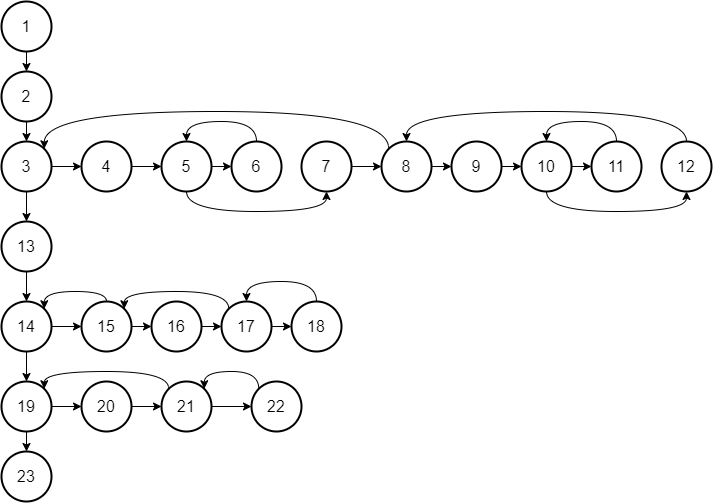
\includegraphics[scale=0.7]{GU.png}
	\caption{Граф управления}
	\label{GU}
\end{figure}

\section{Информационный граф программы}

\begin{figure}[H]
	\centering
	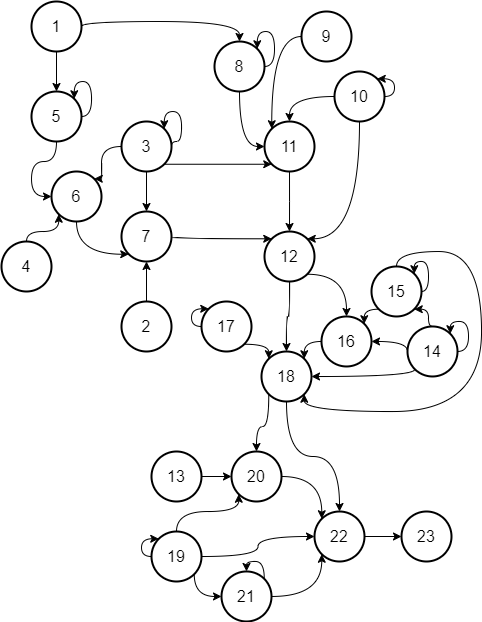
\includegraphics[scale=0.7]{IG.png}
	\caption{Информационный граф}
	\label{IG}
\end{figure}

\section{Операционная история программы}

\begin{figure}[H]
	\centering
	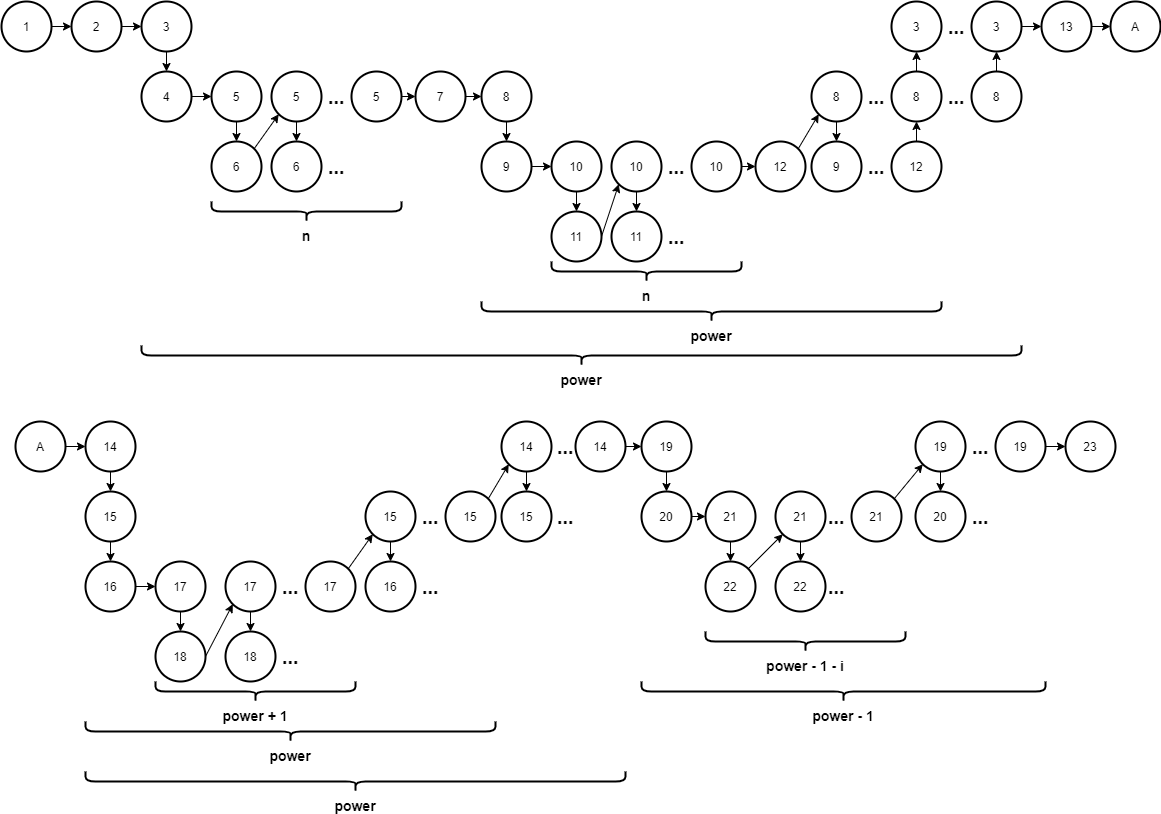
\includegraphics[scale=0.46]{OI.png}
	\caption{Операционная история}
	\label{OI}
\end{figure}

\section{Информационная история программы}

\begin{figure}[H]
	\centering
	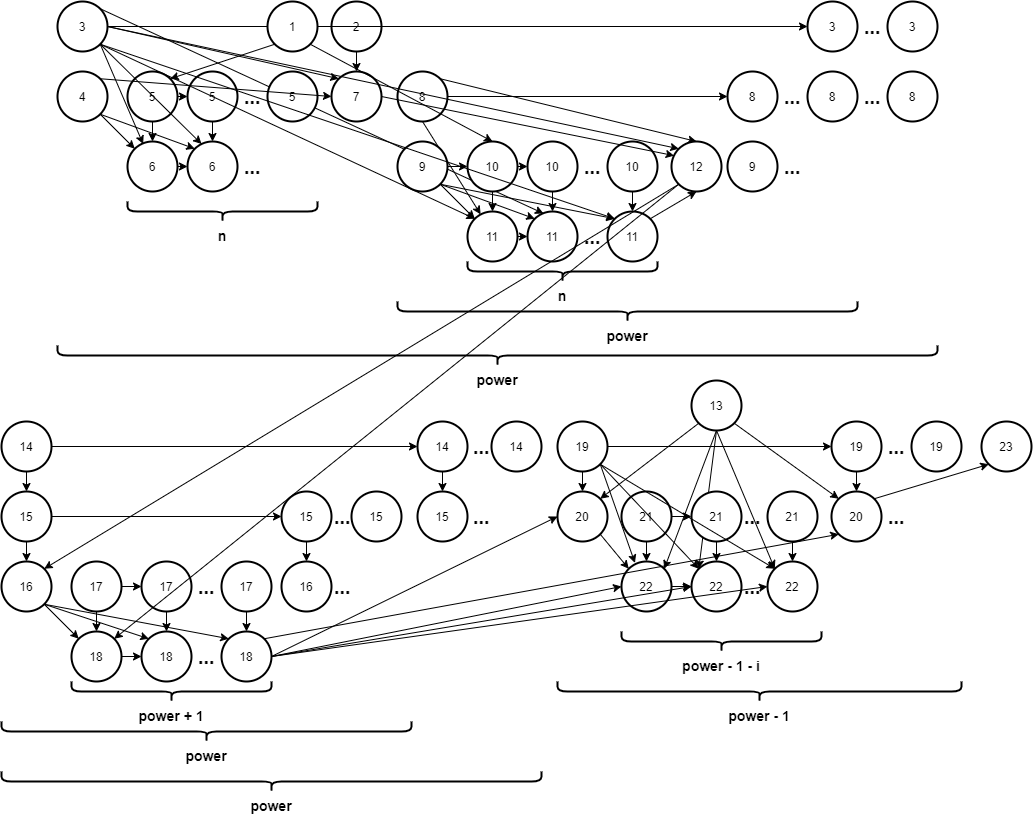
\includegraphics[scale=0.525]{II.png}
	\caption{Информационная история}
	\label{II}
\end{figure}

\end{document}